\documentclass{article} 
\usepackage{polski} 
\usepackage[utf8]{inputenc} 
\usepackage[OT4]{fontenc} 
\usepackage{graphicx,color} 
\usepackage{url} 
\usepackage[pdftex,hyperfootnotes=false,pdfborder={0 0 0}]{hyperref} %za wszystkimi pakietami; pdfborder nie wszedzie tak samo zaimplementowane bo specyfikacja nieprecyzyjna; pod miktex'em po prostu nie widac wtedy ramek

\title{Automatyczna kompozycja kontrapunktu, gatunek I}
\author{Piotr Szachewicz}

\begin{document}
\maketitle

\section{Opis problemu}

Kontrapunkt jest techniką kompozytorską, która polega na prowadzeniu kilku niezależnych linii melodycznych zgodnie z określonymi zasadami harmonicznymi i rytmicznymi~\cite{wikiCounterpoint}.

W innym znaczeniu kontrapunkt oznacza melodię, która jest dokomponowywana do istniejącej już melodii, zwanej \emph{głosem głównym} (\emph{cantus firmus}) \cite{Sikorski}.

Celem pracy jest zaprojektowanie i implementacja programu, który byłby zdolny do automatycznej kompozycji kontrapunktu (gatunek I) zgodnie z opisanymi niżej zasadami dla podanej przez użytkownika melodii \emph{cantus firmus}.

W ramach pracy ograniczono się jedynie do najprostszego rodzaju kontrapunktu, tj. do gatunku I. Przykład kontrapunktu w gatunku I przedstawiono na rysunku~\ref{fig:kontrapunkt_przyklad_gawlas}.

\begin{figure}[htb]
\centering
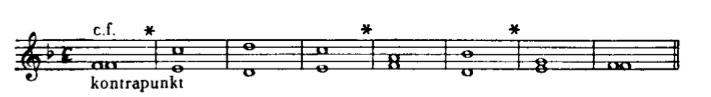
\includegraphics[width=1.0\textwidth]{images/kontrapunkt_przyklad_gawlas.png}
\caption{Przykład kontrapunktu, gatunek I. Górna linia melodyczna oznaczona skrótem \emph{c.f.} to \emph{cantus firmus}, a dolna to linia kontrapunktująca. (Źródło:~\cite{gawlas})}
\label{fig:kontrapunkt_przyklad_gawlas}
\end{figure}

W gatunku I \emph{cantus firmus} składa się z nut o jednakowych wartościach rytmicznych, a jednej nucie z głosu głównego odpowiada dokładnie jedna nuta z głosu kontrapunktującego.

Obowiązują następujące zasady harmoniczne:

\begin{itemize}
\item wszystkie współbrzmienia to konsonanse (pryma czysta, kwinta czysta, oktawa czysta, tercja mała lub wielka, seksta mała lub wielka);
\item rozpoczęcie i zakonczenie to współbrzmienie konsonansu doskonałego (pryma czysta, kwinta czysta, oktawa czysta);
\item wszystkie wertykalne konsonanse doskonałe musza być osiagniete ruchem przeciwnym (oba głosy w przeciwnych kierunkach) lub bocznych (jeden głos porusza się, a drugi jest nieruchomy).
\end{itemize}

Melodia kontrapunktu powinna spełniać następujące zasady melodyczne:

\begin{itemize}
\item przeważają kroki (ruch o sekunde małą lub wielką);
\item przeważa ruch przeciwny (oba głosy powinny poruszać się w przeciwnych kierunkach);
\item niedozwolone są skoki melodii o: tryton, septymę wielką lub małą.
\end{itemize}

Powyższe zasady są zasadami ścisłymi, które powinny obowiązywać dla każdego kontrapunktu. Poza zasadami ścisłymi wyróżnia się również zasady swobodne, które mają mniejszą wagę, np.:

\begin{itemize}
\item mieszaj konsonanse doskonałe (pryma czysta, kwinta czysta, oktawa czysta) i niedoskonałe (tercje, seksty);
\item unikaj prymy czystej w pierwszym i ostatnim współbrzmieniu;
\item unikaj skoku w obu głosach na raz;
\item po dużym skoku powinna nastąpić zmiana kierunku melodii i kroki sekundowe;
\item na przestrzeni 10-20 dźwieków głosu kontrapunktujacego z należy wykorzystać cały zakres dostępnej skali.
\end{itemize}

Dla uproszczenia problemu implementacja oparta zostanie jedynie na zasadach ścisłych.

\section{Implementacja}

Implementacja składa się z następujących modułów:
\begin{itemize}
\item generatora,
\item funkcji oceniającej,
\item algorytmu przeszukiwania.
\end{itemize}

Moduły te zostaną omówione w poniższych podrozdziałach.

\subsection{Generator}

Celem generatora jest wygenerowanie wszystkich możliwych kontrapunktów, które będą zgodne z przedstawionymi powyżej zasadami ścisłymi dotyczącymi harmonii.
Ponadto uwzględnia on skalę dźwięków, z których może składać się kontrapunkt.

Algorytm generatora działa następująco:
\begin{enumerate}
\item Dla każdej nuty w \emph{cantus firmus} obliczane są wysokości dźwięków, które są odległe od niej o konsonse doskonałe i niedoskonałe. Dla każdej nuty \emph{głosu głównego} obliczany i przechowywany jest zbiór dozwolonych dźwięków kontrapunktu.
\item Z obliczonych zbiorów usuwane są dźwięki, które nie należą do zdefiniowanej skali.
\item Zbiór możliwych melodii, które generator jest w stanie wygenerować jest równy iloczynowi kartezjańskiemu zbiorów obliczonych w punkcie 1. (Jest to przestrzeń dozwolonych rozwiązań problemu).
\end{enumerate}

\subsection{Funkcja oceniająca}

Funkcja oceniająca przypisuje każdemu kontrapunktowi liczbę punktów. Podczas oceniania uwzględniane są jedynie zasady ścisłe dotyczące melodii -- nie jest konieczne uwzględnianie zasad dotyczących harmonii, gdyż zasady te uwzględniane są podczas pracy generatora.

Melodia analizowana jest nuta po nucie. Złamanie którejś z zasad powoduje odjęcie odpowiedniej ilości punktów (zależnej od zasady) od puli punktów danego kontrapunktu. W najlepszym przypadku, jeżeli nie zostanie złamana żadna zasada, kontrapunkt może uzyskać maksymalnie $0$ punktów.

\subsection{Algorytm przeszukiwania}

W programie zaimplementowane są dwa algorytmy przeszukiwania przeszukiwanie pełne oraz przeszukiwanie przy użyciu algorytmu genetycznego.

\subsubsection{Pełne przeszukiwanie}

Przeszukiwanie pełne polega na przeglądnięciu i ocenie kolejno wszystkich kontrapunktów wygenerowanych przez generator. Do zbioru końcowego, który jest pokazywany użytkownikowi, wybierany jest podzbiór kontrapunktów, który uzyskał najwyższą liczbę punktów (możliwe jest również przestawienie programu w tryb poszukiwania zbioru kontrapunktów o najgorszej liczbie punktów).

\subsubsection{Algorytm genetyczny}

W programie zaimplementowano algorytm genetyczny przy użyciu biblioteki ECJ \cite{ecjManual, ecjTutorials}.

Algorytm genetyczny zastosowany w programie przebiega następująco:

\begin{enumerate}
\item Losowana jest pewna populacja początkowa kontrapunktów ze zbioru możliwych kontrapunktów generowanych przez generator. Wielkość populacji można ustawić przy pomocy parametru \emph{population size}.
\item Każdemu osobnikowi przypisywana jest ocena uzyskana przy pomocy funkcji oceniającej.
\item Wybierane są osobniki, które mają wziąć udział w procesie reprodukcji. Proces selekcji odbywa się w następujący sposób:
	\begin{enumerate}
		\item losowanych jest $n$ osobników z populacji (gdzie $n$ jest wielkością turnieju, którą można ustawić przy użyciu GUI);
		\item do reprodukcji wybierany jest ten z wylosowanych osobników, który ma najwyższą ocenę.
	\end{enumerate}

\item Następnie osobniki, które zostały wybrane w procesie selekcji, są krzyżowane. Krzyżowanie może przebiegać według jednego z następujących algorytmów (do wyboru w GUI):

	\begin{itemize}
		\item \emph{one-point crossover} -- dane są dwa osobniki, będące ciągiem nut, następnie losowo wybierane jest miejsce, w którym je rozcinamy. W wyniku operacji krzyżowania powstają dwa osobniki:
			\begin{itemize}
				\item składający się z nut 1 osobnika z lewej strony punktu krzyżowania i nut 2 osobnika z prawej strony punktu krzyżowania;
				\item składający się z nut 2 osobnika z lewej strony punktu krzyżowania i nut 1 osobnika z prawej strony punktu krzyżowania.
			\end{itemize}
		\item \emph{two-point crossover} -- wybierane są losowo dwa punkty krzyżowania, pomiędzy osobnikami wymieniana jest część nut pomiędzy tymi punktami.
		\item \emph{uniform crossover} -- dla każdej nuty losowane jest (zgodnie z prawdopodobieństwem \emph{note crossover probability}), czy ma ona zostać wymieniona z drugim osobnikiem.
	\end{itemize}

\item W wyniku krzyżowania powstaje nowa populacja, o takiej samej liczności jak populacja początkowa. Osobniki z tej populacji poddawane są mutacjom, tj. wprowadzane są drobne losowe zmiany w ich genotypach. Oznacza to, że każda nuta należąca do genotypu osobnika może losowo zmienić się na dowolną inną (ale taką, która jest dozwolona przez generator) z pewnym prawdopodobieństwem \emph{note mutation probability}. 

\item Algorytm powtarzany jest od punktu $2$, dopóki liczba kroków algorytmu nie będzie równa \emph{number of generations}.
\end{enumerate}

\section{Testy}

Podczas testów porównano wyniki i czasy działania algorytmu pełnego przeszukiwania z algorytmem genetycznym, a także sprawdzono wpływ różnych ustawień parametrów algorytmu genetycznego na jakość uzyskiwanych rozwiązań.

\subsection{Wygenerowane kontrapunkty}

Testy przeprowadzono przy użyciu \emph{cantus firmus} przedstawionego na rysunku~\ref{fig:testowy_cantus_firmus}.

\begin{figure}[htb]
\centering
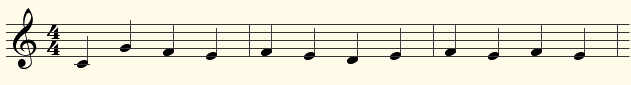
\includegraphics[width=1.0\textwidth]{images/testowy_cantus_firmus.png}
\caption{\emph{Cantus firmus} użyty do testów}
\label{fig:testowy_cantus_firmus}
\end{figure}

W wyniku pełnego przeszukania przestrzeni rozwiązań w poszukiwaniu najlepiej ocenianych kontrapunktów znaleziono kontrapunkty przedstawione na rysunku~\ref{fig:najlepsze_kontrapunkty}. Po przełączeniu odpowiedniej opcji w programie wyszukano również najgorzej ocenione kontrapunkty (rysunek~\ref{fig:najgorsze_kontrapunkty}).

\begin{figure}[htb]
\centering
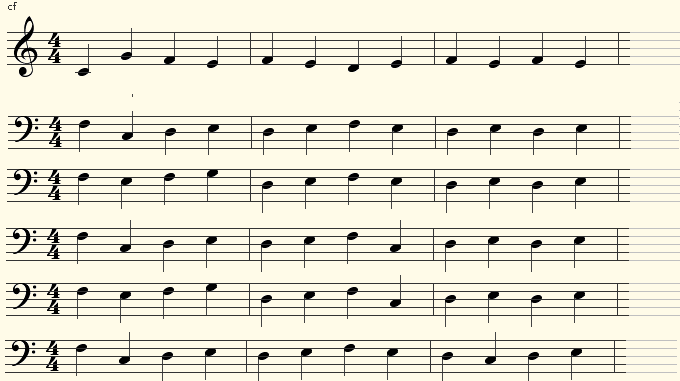
\includegraphics[width=1.0\textwidth]{images/najlepsze_kontrapunkty.png}
\caption{Najlepsze kontrapunkty uzyskane w wyniku testów. Uzyskały one odpowiednio -7, -7, -8, -8 oraz -10 punktów.}
\label{fig:najlepsze_kontrapunkty}
\end{figure}

\begin{figure}[htb]
\centering
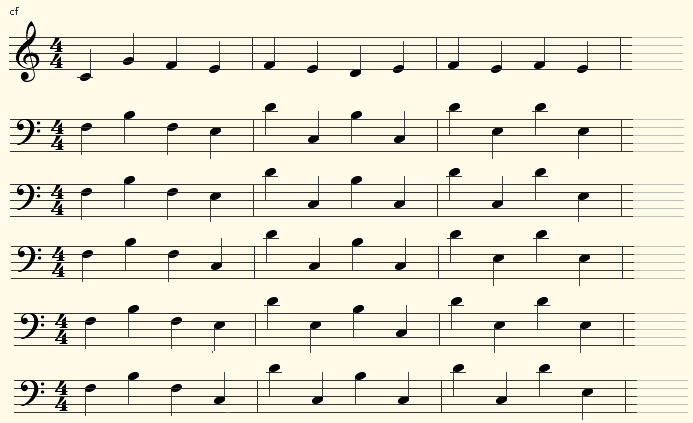
\includegraphics[width=1.0\textwidth]{images/najgorsze_kontrapunkty.png}
\caption{Najgorsze kontrapunkty uzyskane w wyniku testów. Uzyskały one odpowiednio -710, -704, -696, -694 oraz 690 punktów.}
\label{fig:najgorsze_kontrapunkty}
\end{figure}

\subsection{Porównanie pełnego przeszukiwania i algorytmu genetycznego}

Podczas testów zmierzono czasy wykonania oraz jakości otrzymanych rozwiązań uzyskanych przy pomocy pełnego przeszukiwania oraz algorytmu genetycznego w zależności od długości kontrapunktu (którego długość w przypadku rozważanego gatunku zawsze jest równa długości \emph{cantus firmus}). 

Do testów tych użyto \emph{cantus firmus} przedstawionego w poprzednim podrozdziale, wycinając z nich w razie potrzeby odpowiednią liczbę nut. Dla przykładu, robiąc pomiary dla \emph{cantus firmus} o długości $4$ nut, wycinano $4$ pierwsze nuty z poprzednio przedstawionego głosu głównego.

Otrzymane wyniki przedstawiono w tabeli~\ref{tab:wyniki1} oraz na rysunkach~\ref{fig:liczba_nut_a_mozliwe_rozwiazania}-\ref{fig:liczba_nut_a_jakosc}.

\begin{table}
\begin{center}
  \begin{tabular}{ | p{0.8cm} | p{2.8cm} | p{1.4cm} | p{1.4cm} | p{1.4cm} | p{1.4cm} | }
    \hline
    \multicolumn{2}{|c|}{} & \multicolumn{2}{|c|}{pełne przeszukiwanie} & \multicolumn{2}{|c|} {algorytm genetyczny}\\ \hline \hline

	liczba nut & liczba możliwych rozwiązań & czas wykonania $[ms]$& najlepsza ocena & czas wykonania $[ms]$& najlepsza ocena \\ \hline \hline
	4 & 120 & 4 & -2 & 43 & -2 \\ \hline
	5 & 300	& 8 & 0 & 30 & 0 \\ \hline
	6 & 2400 & 192 & -2 & 50 & -2 \\ \hline
	7 & 12000 & 279 & -4 & 50 & -4 \\ \hline
	8 & 48000 & 1444 & -2 & 76 & -2 \\ \hline
	9 & 120000 & 3471 & -4 & 63 & -8 \\ \hline
	10 & 960000 & 30843 & -2 & 73 & -14 \\ \hline
	11 & 2400000 & 87607 & -4 & 90 & -16 \\ \hline
	12 & 19200000 & 836272 & -7 & 93 & -23 \\ \hline
  \end{tabular}
  \caption{Liczba możliwych rozwiązań oraz czasy wykonania algorytmów i najlepsza ocena uzyskana przy użyciu pełnego przeszukiwania oraz algorytmu genetycznego w zależności od długości \emph{cantus firmus}}
  \label{tab:wyniki1}
  \end{center}
\end{table}

\begin{figure}[htb]
\centering
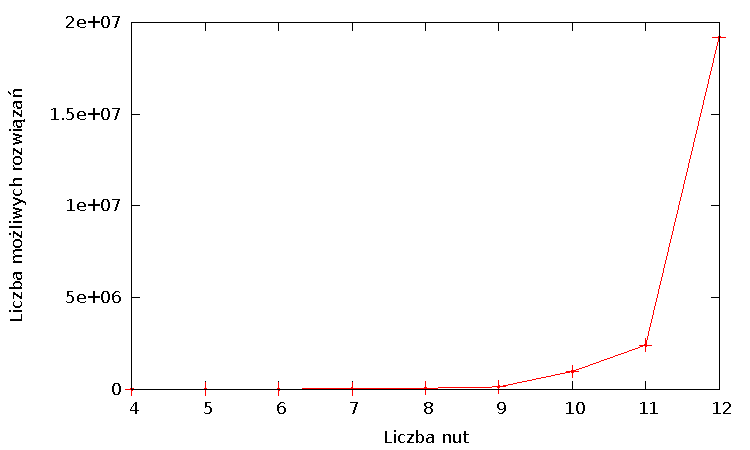
\includegraphics[width=1.0\textwidth]{images/liczba_nut_a_mozliwe_rozwiazania.pdf}
\caption{Wykres przedstawiający liczbę możliwych rozwiązań w zależności od długości \emph{cantus firmus}.}
\label{fig:liczba_nut_a_mozliwe_rozwiazania}
\end{figure}

\begin{figure}[htb]
\centering
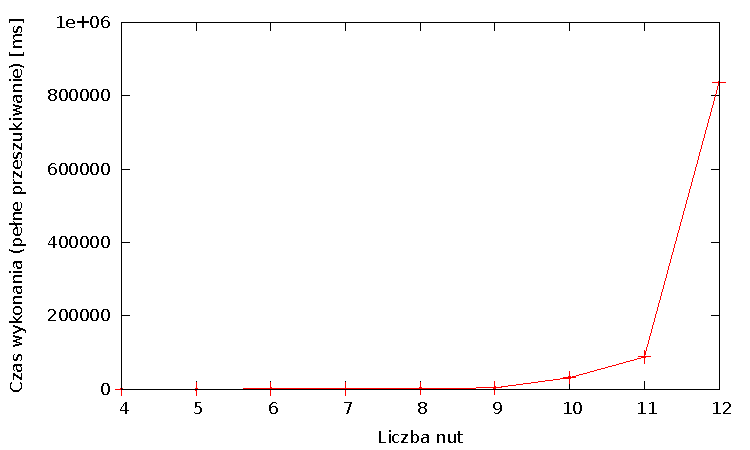
\includegraphics[width=1.0\textwidth]{images/liczba_nut_a_czas_FS.pdf}
\caption{Wykres przestawia czas pełnego przeszukiwania w zależności od długości \emph{cantus firmus}.}
\label{fig:liczba_nut_a_czas_FS}
\end{figure}

\begin{figure}[htb]
\centering
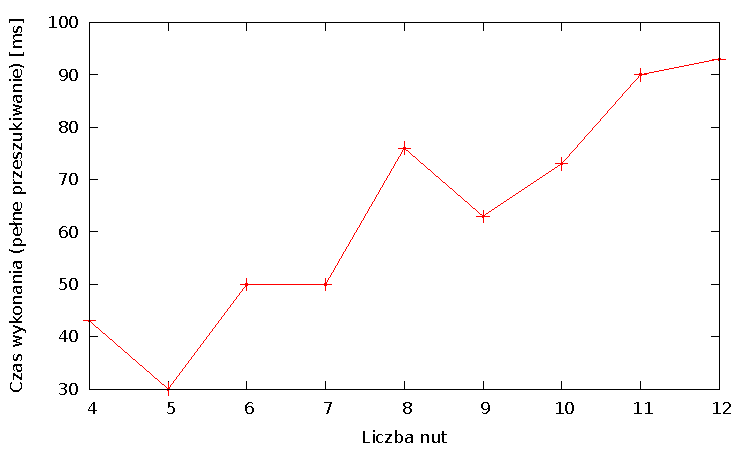
\includegraphics[width=1.0\textwidth]{images/liczba_nut_a_czas_AG.pdf}
\caption{Wykres przestawia czas wykonania algorytmu genetycznego w zależności od długości \emph{cantus firmus}.}
\label{fig:liczba_nut_a_czas_AG}
\end{figure}

\begin{figure}[htb]
\centering
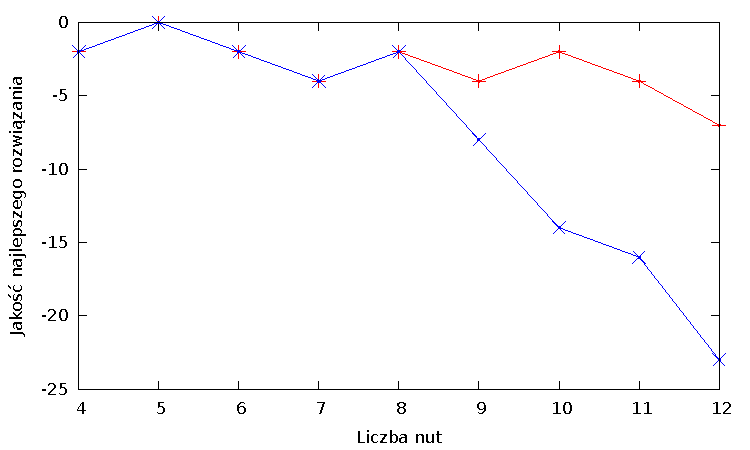
\includegraphics[width=1.0\textwidth]{images/liczba_nut_a_jakosc.pdf}
\caption{Wykres przestawia oceny najlepszych kontrapunktów w zależności od długości \emph{cantus firmus}. Czerwona linia przedstawia oceny uzyskane przy użyciu pełnego przeszukiwania, a niebieska -- przy użyciu algorytmu genetycznego.}
\label{fig:liczba_nut_a_jakosc}
\end{figure}

Na wykresie\ref{fig:liczba_nut_a_mozliwe_rozwiazania} przedstawiono liczbę wszystkich dopuszczonych przez generator rozwiązań w zależności od długości \emph{cantus firmus}. Liczba ta rośnie wykładniczo w zależności od liczby nut w \emph{cantus firmus}. Skutkuje to bardzo długimi czasami wykonania, jeśli użyte zostanie pełne przeszukiwania przestrzeni rozwiązań -- niemożliwe staje się wygenerowanie w rozsądnym czasie kontrapunktu dla długich \emph{cantus firmus}.

W tym wypadku korzystne staje się użycie algorytmu genetycznego -- charakteryzuje się on znacznie krótszym czasem wykonania i rośnie liniowo w zależności od długości kontrapunktu. Ponadto, na czas wykonania i jakość uzyskiwanych rozwiązań można wpływać manipulując wielkością populacji i liczbą pokoleń.

\clearpage
\subsection{Parametry algorytmu genetycznego a jakość uzyskiwanych rozwiązań.}

Podczas tego testu zbadano wpływ różnych ustawień parametrów algorytmu genetycznego na jakość uzyskiwanych rozwiązań.

Domyślne ustawienia w programie wynosiły:
\begin{itemize}
\item liczba pokoleń - $5$,
\item wielkość populacji - $400$,
\item wielkość turnieju - $2$,
\item rodzaj algorytmu krzyżującego - \emph{one-point crossover},
\item prawdopodobieństwo mutacji pojedynczej nuty - $0.1$.
\end{itemize}

Do każdego testu wybierano jeden parametr i zmieniano jego wartość obserwując, jak zmienia się ocena najlepszego kontrapunktu. Dla każdej wartości parametru wykonano po $10$ pomiarów, które następnie uśredniono.

Otrzymane wyniki przedstawiono w tabelach~\ref{tab:wynik_a_liczba_generacji}-\ref{tab:wynik_a_mutacja}.

\begin{table}
\begin{center}
  \begin{tabular}{ | c || c | c | c | c | c | }
    \hline
	liczba pokoleń & 5 & 7 & 9 & 25 & 50 \\ \hline
	wynik & -21.9 & -20.6 & -18 & -10.9 & -9.6 \\ \hline
  \end{tabular}
  \caption{Uśredniony najlepszy wynik algorytmu genetycznego w zależności od liczby pokoleń.}
  \label{tab:wynik_a_liczba_generacji}
  \end{center}
\end{table}

\begin{table}
\begin{center}
  \begin{tabular}{ | c || c | c | c | c | }
    \hline
	wielkość populacji & 400 & 600 & 800 & 4000 \\ \hline
	wynik & -21.9 & -21.3 & -21.2 & -16 \\ \hline
  \end{tabular}
  \caption{Uśredniony najlepszy wynik algorytmu genetycznego w zależności od wielkości populacji.}
  \label{tab:wynik_a_wielkosc_populacji}
  \end{center}
\end{table}

\begin{table}
\begin{center}
  \begin{tabular}{ | c || c | c | c | c | c | c | c | c | c | c |}
    \hline
	wielkość turnieju & 2 & 3 & 5 & 7 & 9 & 11 & 13 & 15 & 40 & 100 \\ \hline
	wynik & -21.9 & -20.7 & -14.7 & -15.5 & -12.5 & -11.6 & -12.5 & -11 & -10 & -9.7 \\ \hline
  \end{tabular}
  \caption{Uśredniony najlepszy wynik algorytmu genetycznego w zależności od wielkości turnieju.} 
  \label{tab:wynik_a_tournament_size}
  \end{center}
\end{table}

\begin{table}
\begin{center}
  \begin{tabular}{ | p{1.4cm} || c | c | p{1.4cm}  | p{1.4cm}   | p{1.4cm}  | p{1.4cm}  | }
    \hline
	rodzaj krzyżowania & one-point & two-point & uniform (0.05) & uniform (0.1) & uniform (0.3) & uniform (0.5) \\ \hline
	wynik & -21.9 & -23.1 & -25.3 & -24.6 & -26.4 & -26.7 \\ \hline 
  \end{tabular}
  \caption{Uśredniony najlepszy wynik algorytmu genetycznego w zależności od rodzaju algorytmu krzyżującego.}
  \label{tab:wynik_a_crossover}
  \end{center}
\end{table}

\begin{table}
\begin{center}
  \begin{tabular}{ | c || c | c | c | c | c | }
    \hline
	prawdopodobieństwo mutacji & 0.01 & 0.05 & 0.1 & 0.2 & 0.3 \\ \hline
	wynik & -23.8 & -23.1 & -21.9 & -24.5 & -25.2 \\ \hline 
  \end{tabular}
  \caption{Uśredniony najlepszy wynik algorytmu genetycznego w zależności od prawdopobieństwa mutacji pojedynczej nuty.}
  \label{tab:wynik_a_mutacja}
  \end{center}
\end{table}

Z przedstawionych wyników można wywnioskować, że polepszenie otrzymywanych wyników można łatwo uzyskać zwiększając liczbę pokoleń - im więcej razy krzyżuje i mutuje się osobniki, tym większa jest szansa na otrzymanie osobnika bardziej optymalnego.

Z kolei zwiększanie wielkości populacji powoduje nieco wolniejsze polepszanie otrzymywanych wyników. Spowodowane jest ono głównie większym prawdopodobieństwem wylosowania lepszych osobników w populacji, ale warto zauważyć, że również w tym wypadku zwiększa się również liczba krzyżowań osobników.

Bardzo dobre wyniki uzyskano, jeśli zwiększano wielkość turnieju. Zwiększenie tego parametru powoduje, że więcej osobników jest losowanych do pojedynczej rywalizacji o możliwość reprodukcji. Skutkiem ubocznym jest zmniejszenie szans słabszych osobników na uczestnictwo w procesie krzyżowania, a polepszenie tych szans dla lepszych osobników.

Z kolei zmiana algorytmu krzyżującego oraz prawdopodobieństwa mutacji z domyślnych wartości nie przynosiła poprawy otrzymywanych wyników.

\subsection{Korekta parametrów algorytmu genetycznego}

Dodatkowo, przetestowano również, jak będzie działać algorytm genetyczny przy zmienionych parametrach. Najważniejszą zmianą była zmiana proporcji wielkości populacji do liczby pokoleń.

Zaimplementowano również możliwość ustalenia prawdopodobieństwa, z jakim obiekt zostanie poddany krzyżowaniu (jeżeli nie zostaje poddany krzyżowaniu, ulega jedynie mutacjom).

Testy opisane w tym rozdziale przeprowadzono na następujących wartościach parametrów:
\begin{itemize}
\item liczba pokoleń - $100$,
\item wielkość populacji - $20$,
\item wielkość turnieju - $5$,
\item rodzaj algorytmu krzyżującego - \emph{one-point crossover},
\item prawdopodobieństwo krzyżowania - $0.3$,
\item prawdopodobieństwo mutacji pojedynczej nuty - $0.1$.
\end{itemize}

Dla każdej długości \emph{cantus firmus} przeprowadzono $10$ testów i pomiary uśredniono. Uzyskane wyniki przedstawiono w tabeli~\ref{tab:wyniki2} oraz na rysunku~\ref{fig:liczba_nut_a_jakosc_poprawki}.

Na podstawie poniższych danych można zauważyć, że korzystne jest w tym wypadku znaczne zwiększenie liczby pokoleń kosztem wielkości populacji.

\begin{table}
\begin{center}
  \begin{tabular}{ | c | c | } 
    \hline
	liczba nut & najlepsza ocena \\ \hline \hline
	4 & -2.6 \\ \hline
	5 & 0.0 \\ \hline
	6 & -4.6 \\ \hline
	7 & -6.4 \\ \hline
	8 & -3.6 \\ \hline
	9 & -5.2 \\ \hline
	10 & -7.0 \\ \hline
	11 & -4.6 \\ \hline
	12 & -12.2 \\ \hline
  \end{tabular}
  \caption{Najlepsza ocena uzyskana przy użyciu algorytmu genetycznego przy zmienionych parametrach w zależności od długości \emph{cantus firmus}}
  \label{tab:wyniki2}
  \end{center}
\end{table}

\begin{figure}[htb]
\centering
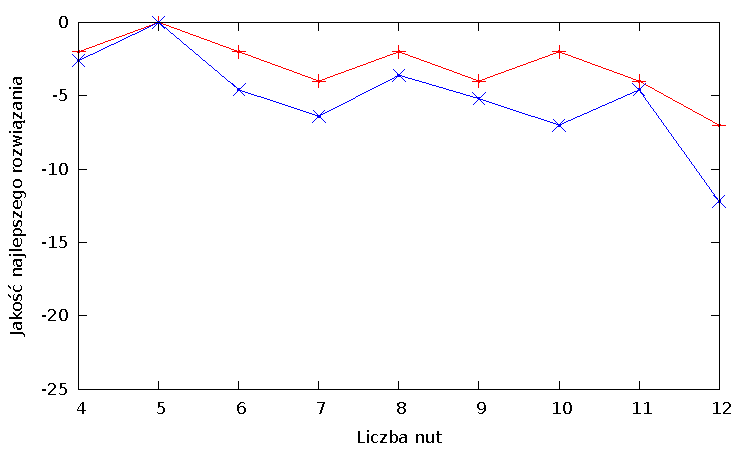
\includegraphics[width=1.0\textwidth]{images/liczba_nut_a_jakosc_poprawki.pdf}
\caption{Wykres przestawia oceny najlepszych kontrapunktów w zależności od długości \emph{cantus firmus} dla nowych wartości parametrów algorytmu genetycznego. Czerwona linia przedstawia oceny uzyskane przy użyciu pełnego przeszukiwania, a niebieska -- przy użyciu algorytmu genetycznego.}
\label{fig:liczba_nut_a_jakosc_poprawki}
\end{figure}


\section{Wnioski}

W ramach niniejszej pracy zaimplementowano i zbadano program do automatycznego komponowania kontrapunktu w I gatunku.

W pierwszej kolejności zaimplementowano algorytm przeszukujący wszystkie możliwe rozwiązania problemu w poszukiwaniu najlepszego kontrapunktu. Niestety, z powodu wykładniczo rosnącej przestrzeni rozwiązań, okazał się on przydatny jedynie dla bardzo krótkich kontrapunktów, składających się z 9-10 nut.

W kolejnym podejściu zaimplementowano do przeszukiwania przestrzeni rozwiązń algorytm genetyczny. Jego użycie pozwoliło na znalezienie w bardzo krótkim czasie dość dobrych (choć nie zawsze optymalnych) wyników dla badanego \emph{cantus firmus}.

Dodatkowo, dzięki algorytmu genetycznemu możliwe jest również znajdowanie kontrapunktów dla dużo dłuższych \emph{cantus firmus}. Przy użyciu odpowiednich parametrów możliwe jest zdefiniowanie, jak długo chcemy czekać na rozwiązanie danego problemu.

\clearpage

\bibliography{raport}
\bibliographystyle{plain}

\end{document}

